\documentclass{beamer}

% =====================
% Thème
% =====================
\usetheme{Madrid}
\usecolortheme{default}
\setbeamertemplate{navigation symbols}{} % enlève les icônes

% =====================
% Langue et encodage
% =====================
\usepackage[french]{babel}
\usepackage[T1]{fontenc}
\usepackage{lmodern}


% =====================
% Packages utiles
% =====================
\usepackage{graphicx}
\usepackage{tikz}
\usepackage{booktabs}
\usepackage{pgfplots}
\pgfplotsset{compat=1.18}
\usepackage[table]{xcolor}

% =====================
% Couleurs personnalisées
% =====================
\setbeamercolor{frametitle}{fg=white,bg=myblue}
\definecolor{myblue}{RGB}{40,60,90}
\definecolor{mygray}{RGB}{240,240,240}

\setbeamercolor{structure}{fg=myblue}
\setbeamercolor{frametitle}{fg=white,bg=myblue}
\setbeamercolor{title}{fg=white}

% footer propre
\setbeamertemplate{footline}[frame number]

% =====================
% Infos présentation
% =====================

\author{Thomas Coutant | Benoît Litampha | Auriane Peter}
\institute{
Université Marie \& Louis Pasteur, UFR Sciences et Techniques
}
\title{Projet L3 : PacMan en réseau}
\date{Licence CMI Informatique -- 3\textsuperscript{ème} année \\ 2025--2026}

% =====================
% Document
% =====================
\begin{document}

% ---------------------
% Page de titre
% ---------------------
\begin{frame}
\titlepage


\begin{center}

Encadrant : Julien Bernard\\
\vspace{0.5cm}
\includegraphics[width=0.3\textwidth]{images/logo_univ.jpg}
\hspace{1cm}
\includegraphics[width=0.3\textwidth]{images/logo_ufrst.png}

\vspace{0.5cm}



\end{center}

\end{frame}

% ---------------------
% Plan
% ---------------------
\begin{frame}{Plan}
\tableofcontents
\end{frame}

% ---------------------
% Introduction
% ---------------------
\section{Introduction}

\begin{frame}{Introduction}

\begin{itemize}
\item Contexte du projet
\item Objectifs
\item Organisation
\end{itemize}

\end{frame}

\section{Présentation \& organisation}

\begin{frame}{Git \& discord}

    on a utiliser git pour versionner
    discord pour communiquer entre nous ainsi quavec le tuteur du projet
    de plus on fesait des reunion chaque semaine ou toute sles 2 semaine enfin davoir des retour.
    en parrallele on communiquait quotidiennement entre nous pour definir l'avancer du projet

\end{frame}

\begin{frame}{PacMan}

    copie du rapport

\end{frame}

\begin{frame}{Organisation}

    thomas server
    aurianne client
    benoit les deux + reseau

\end{frame}

\section{Server}

\begin{frame}{Architecture du serveur}

\centering
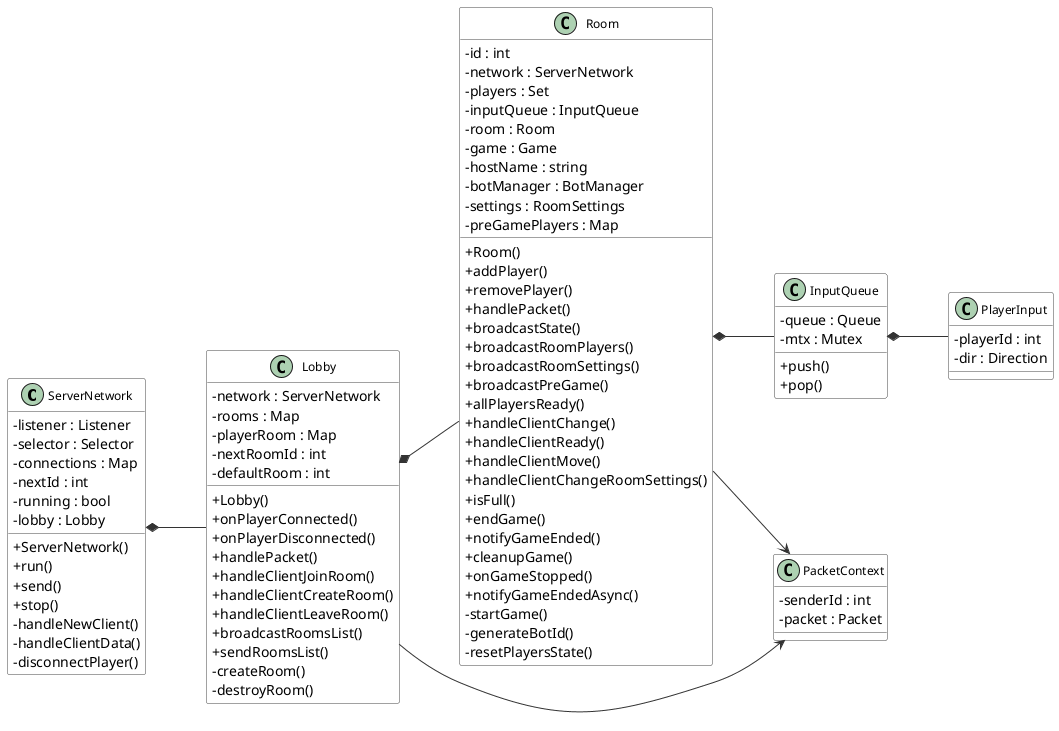
\includegraphics[width=\textwidth,height=0.75\textheight,keepaspectratio]{UML/PacMan_UML_Server_Reseau.png}

\vspace{0.4cm}

Client $\rightarrow$ Server $\rightarrow$ Lobby $\rightarrow$ Room $\rightarrow$ Game

\end{frame}

\begin{frame}{Boucle de jeu}

\textbf{Serveur autoritaire}

\begin{itemize}
    \item Le \textbf{serveur décide de tout}
    \item Les \textbf{clients affichent uniquement l'état reçu}
    \item Permet d'\textbf{éviter la triche} et les désynchronisations
\end{itemize}

\vspace{0.4cm}

\textbf{Tick serveur}

\begin{itemize}
    \item La boucle de jeu fonctionne avec des \textbf{mises à jour périodiques}
    \item Un \textbf{thread serveur} met à jour l'état du jeu :
    \begin{itemize}
        \item positions des joueurs et fantômes
        \item pac-gommes
        \item timers
        \item score et conditions de victoire
    \end{itemize}
\end{itemize}

\vspace{0.4cm}

\textbf{États de la partie}

\begin{itemize}
    \item Avant la partie (préparation)
    \item Partie en cours
    \item Fin de partie
\end{itemize}

\end{frame}
\begin{frame}{IA des fantômes - Principe}

Avoir des fantômes capables de s'adapter au nombre de joueurs et de produire
une forme d'\textbf{intelligence collective}.

\vspace{0.4cm}

\textbf{Inspiration : les fourmis}

\begin{itemize}
    \item Dans la nature, les fourmis utilisent des \textbf{phéromones} pour communiquer.
    \item Chaque fourmi laisse une trace que les autres peuvent suivre.
\end{itemize}

\vspace{0.4cm}

\textbf{Adaptation dans le jeu}

\begin{itemize}
    \item Les entités laissent des \textbf{traces} sur le plateau.
    \item Chaque trace possède :
    \begin{itemize}
        \item une \textbf{intensité} qui diminue avec le temps
        \item un \textbf{propriétaire}
        \item une \textbf{couleur}
    \end{itemize}
    \item \textcolor{red}{Rouge} : Pac-Man \quad | \quad \textcolor{blue}{Bleu} : fantômes
\end{itemize}

\end{frame}

\begin{frame}{IA des fantômes - Prise de décision}

\begin{columns}

\column{0.5\textwidth}

Les fantômes choisissent leur déplacement selon le score :

\[
Score = \textcolor{red}{Attraction} - \textcolor{blue}{Répulsions}
\]

\begin{itemize}
    \item Les traces de \textbf{Pac-Man} créent une \textcolor{red}{attraction}
    \item Les traces des \textbf{fantômes} créent une \textcolor{blue}{répulsion}
    \item La \textcolor{blue}{répulsion} est plus forte pour les \textbf{traces du fantôme lui-même}
\end{itemize}

\column{0.5\textwidth}

\centering
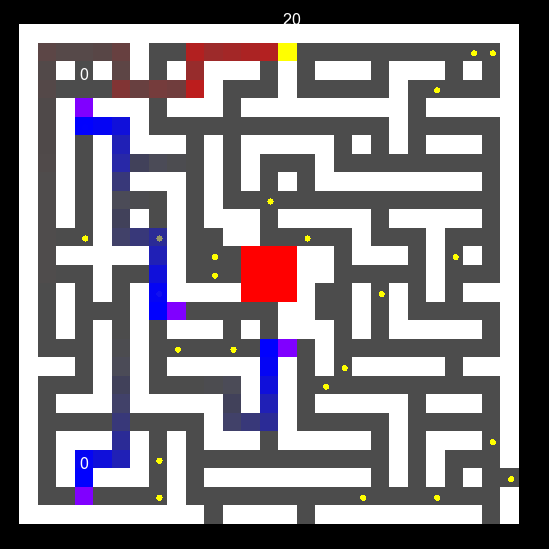
\includegraphics[width=\linewidth]{images/trace.png}

\end{columns}

\end{frame}

\begin{frame}{Génération procédurale du plateau}

\begin{columns}

\column{0.5\textwidth}

\textbf{Variante de l'algorithme de Prim}

\begin{itemize}
    \item Plateau initialement rempli de murs
    \item Choix d'une case de départ
    \item Ajout des murs adjacents dans une liste
    \item Ouverture progressive de murs aléatoires
\end{itemize}

\textbf{Résultat :}
\begin{itemize}
    \item Labyrinthe connexe
    \item Aucune zone isolée
\end{itemize}

\column{0.5\textwidth}

\centering
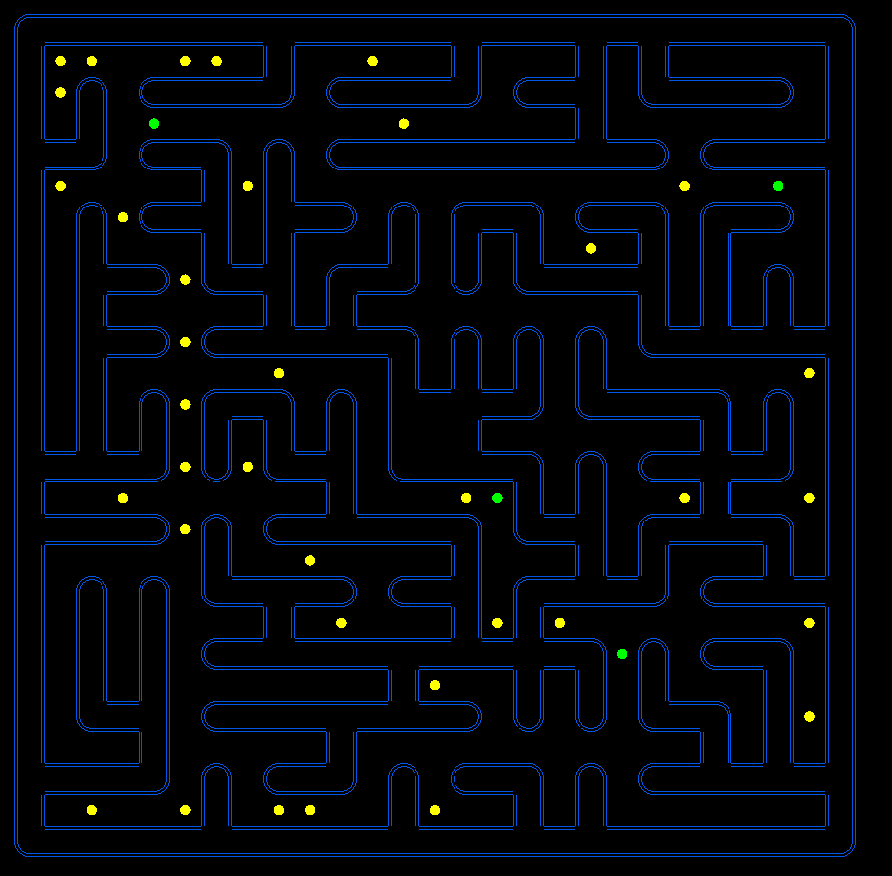
\includegraphics[width=\linewidth]{images/plateau_42_1.png}

\end{columns}

\end{frame}


\begin{frame}{Adaptations pour le gameplay}

\begin{columns}

\column{0.5\textwidth}

\textbf{Contraintes du jeu}

\begin{itemize}
    \item Zone centrale fixe : \textbf{hut $3\times3$}
    \item Vérification de l'accès aux \textbf{coins de départ}
\end{itemize}

\vspace{0.4cm}

\textbf{Améliorations}

\begin{itemize}
    \item Ajout de \textbf{cycles}
    \item Réduction des \textbf{culs-de-sac}
    \item Ajout de \textbf{portails latéraux}
\end{itemize}

\column{0.5\textwidth}

\centering
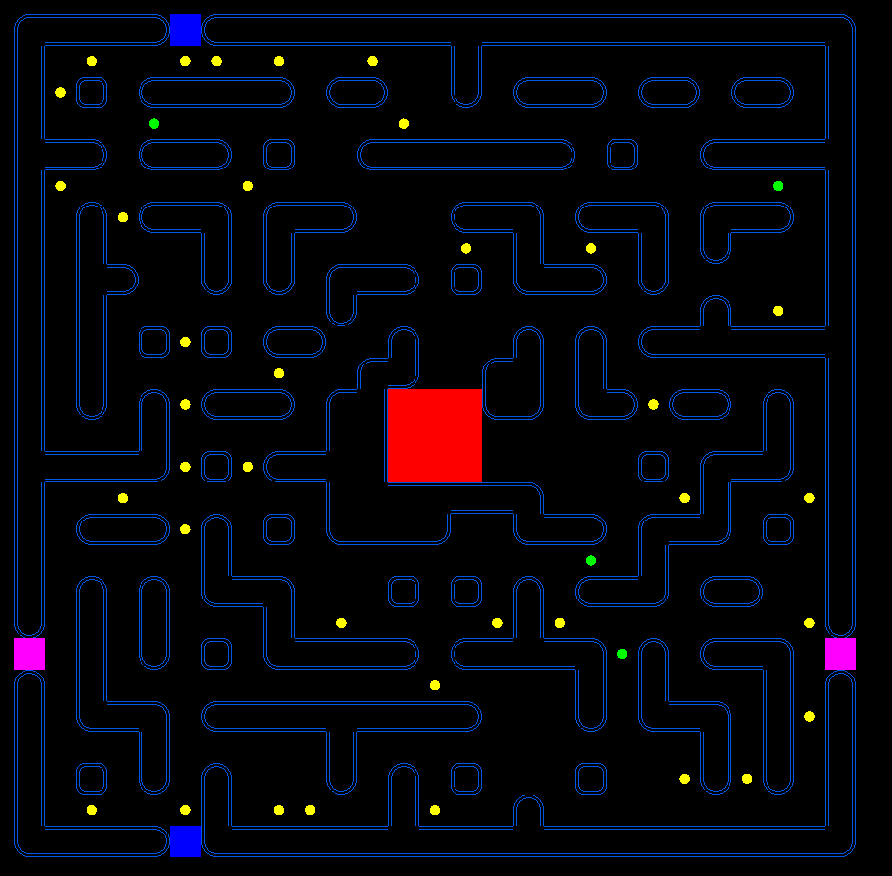
\includegraphics[width=\linewidth]{images/plateau_42_4.png}

\end{columns}

\end{frame}

\section{Client}

\begin{frame}{SceneManager}

    TODO
    
\end{frame}

\begin{frame}{Reception}

    TODO
    
\end{frame}

\begin{frame}{Envoi}

    TODO
    
\end{frame}

\begin{frame}{Input}

    TODO
    
\end{frame}

\begin{frame}{Entité}

    TODO
    
\end{frame}

\section{Reseau}

\begin{frame}{Protocole}

    Communication avec socket
    Choix entre UDP et TCP, TCP choisit pour sa fiabilité\\
    L'ip et le port peuvent être précisé pour le client ou le serveur en ligne de commande\\
    Descrition du fonctionnement de ClientNetwork et ServerNetwork :\\
    - Une socket de comm dans le client, socket de connexion + socket de comm pour chaque client dans le serv\\
    - Thread pour empiler les packets
    
\end{frame}

\begin{frame}{Structures}

    2 types de structure :
    Structures communes contenant les données communes entre client/server\\
    Exemple avec PlayerData\\
    Structures de comm utilisé pour les échanges réseau (ServerXXX = envoyé par le server, ClientXXX = envoyé par le client)
    Exemple avec ServerListPlayersRoom


    
\end{frame}

\begin{frame}{Serialisation/déserialisation}

    Un Operateur | avec un type Archive, gf::packet.is() pour sérialiser, gf::packet.as() pour déserialiser\\
    Switch case avec le type du packet pour l'identifier avec l'id de la structure\\
    Exemple avec ClientMove et ServerListPlayersRoom
    
\end{frame}

\begin{frame}{Exemple concrèt}

    Un exemple concrèt lorsque le server broadcast la liste des joueurs avec ServerListPlayersRoom :\\
    - Le serv récupère les données de chaque joueurs pour construire la structure, sérialisation avec packet.is(), puis envoie à chaque client\\
    - Le client reçoit ce packet et l'empile, puis dans la boucle de jeu dépile et identifie la structure avec gf::Id pour la déserialiser et afficher la liste des joueurs
    
\end{frame}

\section{Conclusion}

\begin{frame}{Conclusion}

    TODO
    
\end{frame}

\section{Démonstration}

\begin{frame}{Démonstration}

    TODO
    
\end{frame}



\end{document}